

\chapter{Single and double scenario, KFold Validation}

Starting with fitting randomly the classifiers, there are some statistics of the data used for the first test: \\
 {\def\arraystretch{1.3} 
 \begin{table}[H] 
\centering 
\begin{tabular}{|l|l|l|} 
\hline 
  &count train  &count test  \\ \hline
mess  &97  &253  \\ \hline
tele  &335  &715  \\ \hline
what  &219  &481  \\ \hline
mess\_mess  &99  &251  \\ \hline
tele\_mess  &113  &237  \\ \hline
what\_mess  &93  &257  \\ \hline
mess\_tele  &89  &261  \\ \hline
what\_tele  &103  &247  \\ \hline
mess\_what  &106  &244  \\ \hline
original  &111  &239  \\ \hline
\end{tabular} 
\end{table} }
\section{Logistic regression results:} 
Confusion matrix with number of sample and with normalization:
 {\def\arraystretch{1.3} 
 \begin{table}[H] 
\centering 
\begin{tabular}{|l|l|l|l|l|l|l|l|l|l|l|} 
\hline 
  &m  &t  &w  &m\_m  &m\_t  &m\_w  &t\_m  &t\_w  &w\_m  &original  \\ \hline
mess  &184  &0  &0  &46  &4  &19  &0  &0  &0  &0  \\ \hline
tele  &0  &710  &0  &0  &0  &0  &0  &5  &0  &0  \\ \hline
what  &0  &0  &419  &0  &0  &0  &0  &0  &58  &4  \\ \hline
mess\_mess  &21  &0  &0  &220  &6  &4  &0  &0  &0  &0  \\ \hline
tele\_mess  &0  &0  &0  &0  &215  &22  &0  &0  &0  &0  \\ \hline
what\_mess  &0  &0  &0  &0  &88  &169  &0  &0  &0  &0  \\ \hline
mess\_tele  &0  &256  &0  &0  &0  &0  &0  &5  &0  &0  \\ \hline
what\_tele  &0  &9  &0  &0  &0  &0  &2  &236  &0  &0  \\ \hline
mess\_what  &0  &0  &191  &0  &0  &0  &0  &1  &52  &0  \\ \hline
original  &0  &0  &0  &0  &0  &0  &0  &0  &0  &239  \\ \hline
\end{tabular} 
\end{table} }

 \begin{figure}[H] 
\centering 
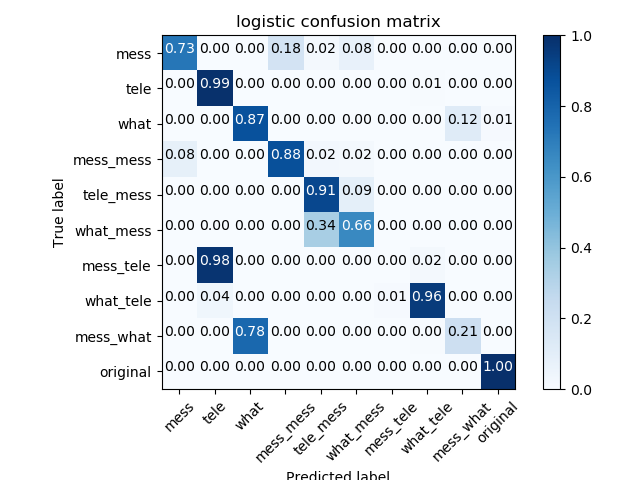
\includegraphics[scale=.6]{images/new_met_lr_initial_single_double_complete.png} 
\caption{logistic regression, last app classified} 
\end{figure} 


Result of the KFold validation with 10 bins:
 {\def\arraystretch{1.3} 
 \begin{table}[H] 
\centering 
\begin{tabular}{|l |l |l |l |l |l |l |l |l |l |}  
\hline 
0.8029&
0.7810&
0.7810&
0.7737&
0.7372&
0.7353&
0.7059&
0.8162&
0.7721&
0.7794\\ \hline  

\end{tabular} 
\end{table} }

The mean is : 0.768474\section{Linear Support Vector Machine results:} 
Confusion matrix with number of sample and with normalization:
 {\def\arraystretch{1.3} 
 \begin{table}[H] 
\centering 
\begin{tabular}{|l|l|l|l|l|l|l|l|l|l|l|} 
\hline 
  &m  &t  &w  &m\_m  &m\_t  &m\_w  &t\_m  &t\_w  &w\_m  &original  \\ \hline
mess  &192  &0  &0  &36  &5  &20  &0  &0  &0  &0  \\ \hline
tele  &0  &715  &0  &0  &0  &0  &0  &0  &0  &0  \\ \hline
what  &0  &0  &409  &0  &0  &0  &0  &0  &68  &4  \\ \hline
mess\_mess  &39  &0  &0  &204  &6  &2  &0  &0  &0  &0  \\ \hline
tele\_mess  &0  &0  &0  &0  &221  &16  &0  &0  &0  &0  \\ \hline
what\_mess  &0  &0  &0  &0  &66  &191  &0  &0  &0  &0  \\ \hline
mess\_tele  &0  &261  &0  &0  &0  &0  &0  &0  &0  &0  \\ \hline
what\_tele  &0  &5  &0  &0  &0  &0  &0  &242  &0  &0  \\ \hline
mess\_what  &0  &0  &174  &0  &0  &0  &0  &1  &69  &0  \\ \hline
original  &0  &0  &0  &0  &0  &0  &0  &0  &0  &239  \\ \hline
\end{tabular} 
\end{table} }

 \begin{figure}[H] 
\centering 
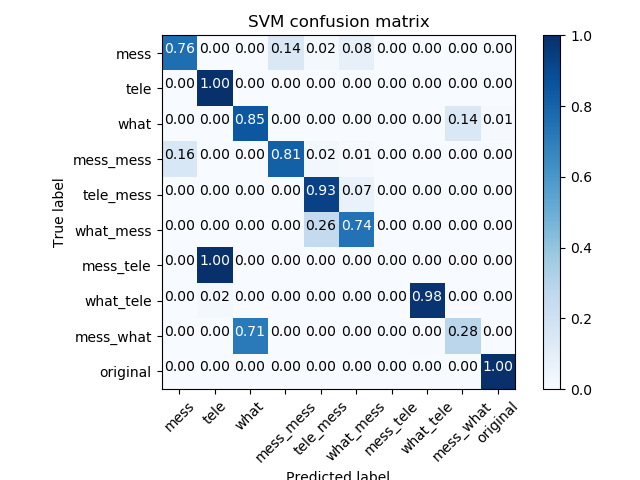
\includegraphics[scale=.6]{images/new_met_lsvm_initial_single_double_complete.png} 
\caption{linear SVM, last app classified} 
\end{figure} 


Result of the KFold validation with 10 bins:
 {\def\arraystretch{1.3} 
 \begin{table}[H] 
\centering 
\begin{tabular}{|l |l |l |l |l |l |l |l |l |l |}  
\hline 
0.8102&
0.7956&
0.7737&
0.8175&
0.7664&
0.8015&
0.7426&
0.8015&
0.8162&
0.7941\\ \hline  

\end{tabular} 
\end{table} }

The mean is : 0.791939\section{Random forest results:} 
Confusion matrix with number of sample and with normalization:
 {\def\arraystretch{1.3} 
 \begin{table}[H] 
\centering 
\begin{tabular}{|l|l|l|l|l|l|l|l|l|l|l|} 
\hline 
  &m  &t  &w  &m\_m  &m\_t  &m\_w  &t\_m  &t\_w  &w\_m  &original  \\ \hline
mess  &192  &0  &0  &36  &3  &19  &0  &0  &3  &0  \\ \hline
tele  &0  &609  &0  &0  &0  &0  &103  &3  &0  &0  \\ \hline
what  &0  &0  &362  &0  &0  &0  &0  &0  &115  &4  \\ \hline
mess\_mess  &50  &0  &0  &189  &8  &3  &0  &0  &1  &0  \\ \hline
tele\_mess  &1  &0  &0  &5  &211  &20  &0  &0  &0  &0  \\ \hline
what\_mess  &10  &0  &7  &17  &25  &196  &0  &0  &2  &0  \\ \hline
mess\_tele  &0  &199  &0  &0  &0  &0  &60  &2  &0  &0  \\ \hline
what\_tele  &0  &5  &0  &0  &0  &0  &1  &241  &0  &0  \\ \hline
mess\_what  &1  &0  &182  &0  &0  &0  &0  &0  &61  &0  \\ \hline
original  &0  &0  &5  &1  &0  &0  &0  &0  &0  &233  \\ \hline
\end{tabular} 
\end{table} }

 \begin{figure}[H] 
\centering 
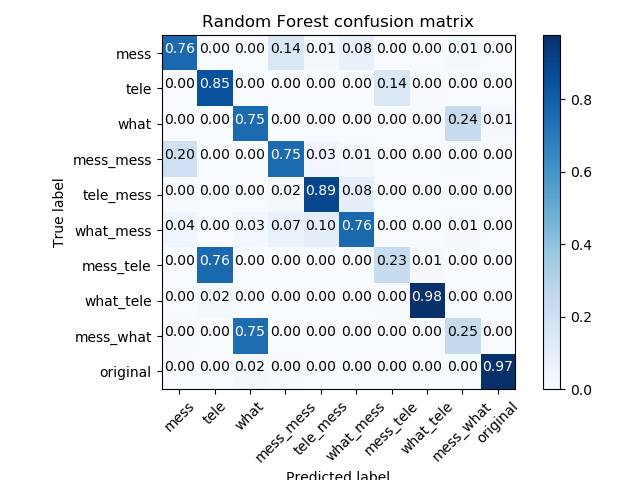
\includegraphics[scale=.6]{images/new_met_rf_initial_single_double_complete.png} 
\caption{random forest, last app classified} 
\end{figure} 


Result of the KFold validation with 10 bins:
 {\def\arraystretch{1.3} 
 \begin{table}[H] 
\centering 
\begin{tabular}{|l |l |l |l |l |l |l |l |l |l |}  
\hline 
0.7591&
0.7664&
0.7007&
0.7445&
0.6496&
0.8309&
0.7206&
0.7647&
0.6618&
0.7574\\ \hline  

\end{tabular} 
\end{table} }

The mean is : 0.735573